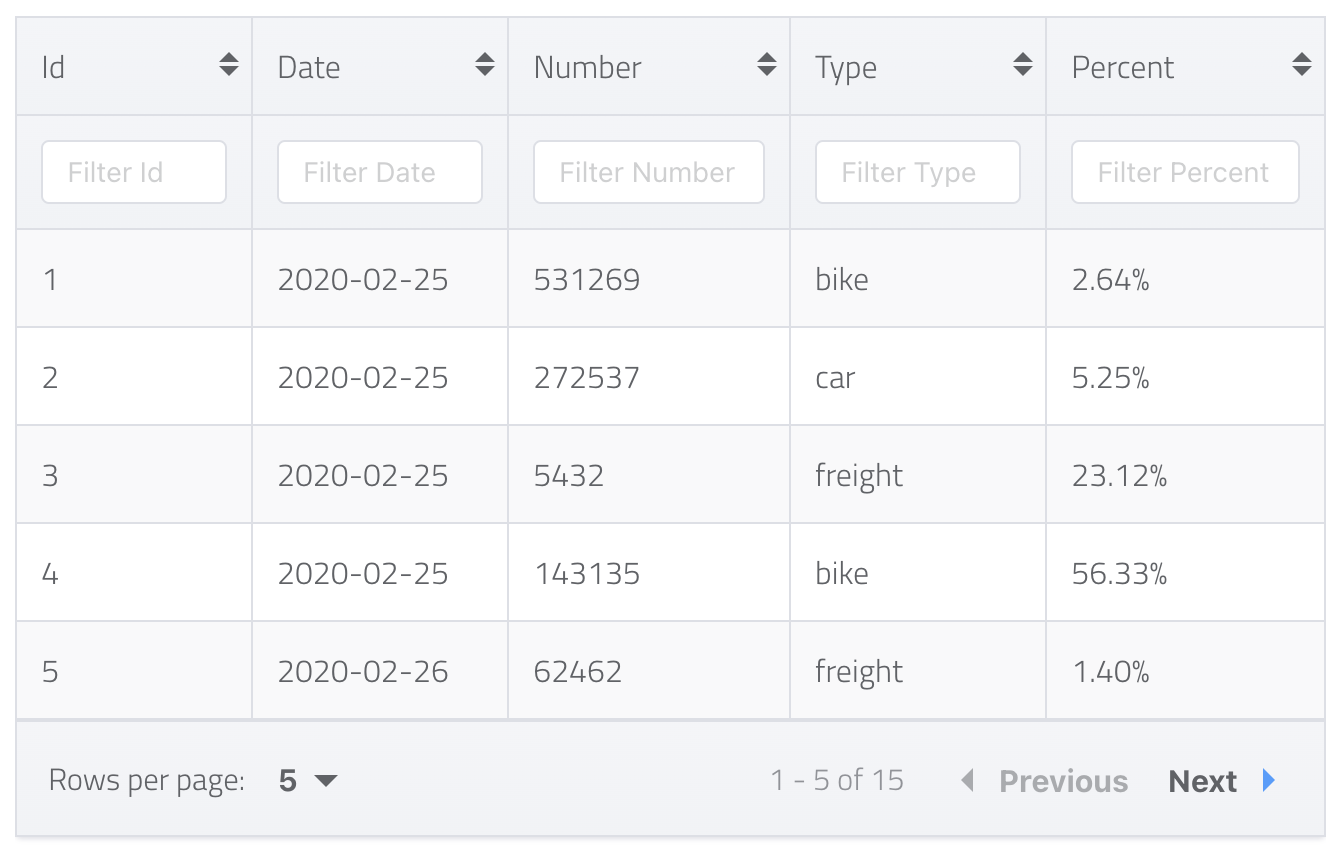
\includegraphics{assets/table.png} \emph{Table Viewer}

The Table viewer is able to display csv files clearly.

\hypertarget{usage}{%
\subsection{Usage}\label{usage}}

The table viewer can only be included as panels in \textbf{Dashboards}.
See Dashboard documentation for general tips on creating dashboard
configurations.

\begin{itemize}
\tightlist
\item
  Each table viewer panel is defined inside a \textbf{row} in a
  \texttt{dashboard-*.yaml} file.
\item
  Use panel \texttt{type:\ csv} in the dashboard configuration.
\item
  Standard title, description, and width fields define the frame.
\end{itemize}

\begin{center}\rule{0.5\linewidth}{0.5pt}\end{center}

\hypertarget{sample-dashboard.yaml-config-snippet}{%
\subsubsection{Sample dashboard.yaml config
snippet}\label{sample-dashboard.yaml-config-snippet}}

\begin{Shaded}
\begin{Highlighting}[]
\FunctionTok{layout}\KeywordTok{:}
\AttributeTok{  }\FunctionTok{row1}\KeywordTok{:}
\AttributeTok{    }\KeywordTok{{-}}\AttributeTok{ }\FunctionTok{type}\KeywordTok{:}\AttributeTok{ }\StringTok{\textquotesingle{}csv\textquotesingle{}}
\AttributeTok{      }\FunctionTok{title}\KeywordTok{:}\AttributeTok{ Example Title}
\AttributeTok{      }\FunctionTok{dataset}\KeywordTok{:}\AttributeTok{ }\StringTok{\textquotesingle{}data.csv\textquotesingle{}}
\AttributeTok{      }\FunctionTok{enableFilter}\KeywordTok{:}\AttributeTok{ }\CharTok{true}
\AttributeTok{      }\FunctionTok{hide}\KeywordTok{:}\AttributeTok{ }\KeywordTok{[}\AttributeTok{bike}\KeywordTok{,}\AttributeTok{ car}\KeywordTok{]}
\AttributeTok{      }\FunctionTok{show}\KeywordTok{:}\AttributeTok{ }\KeywordTok{[}\AttributeTok{bus}\KeywordTok{]}
\AttributeTok{      }\FunctionTok{showAllrows}\KeywordTok{:}\AttributeTok{ }\CharTok{false}
\end{Highlighting}
\end{Shaded}

\begin{center}\rule{0.5\linewidth}{0.5pt}\end{center}

\hypertarget{table-viewer-properties}{%
\subsubsection{Table viewer properties}\label{table-viewer-properties}}

Table viewer properties:

\textbf{dataset:} String. The filepath containing the csv-file.

\textbf{enableFilter:} true/false. This option could be used to filter
columns. This option adds a filter mask to each column. The default
setting is false.

\textbf{hide:} Array of strings. List of column names that should be
ignored.

\textbf{show:} Array of strings. List of column names that should be
displayed. If the hide and show option are in the .yaml file the hide
option will be ignored.

\textbf{showAllRows:} true/false. This option defines whether the whole
table should be displayed or if there are several pages. The default
setting is false.
